% ===============================
%          Chapter 1B.1
%  The Principles of Circulation
%     Created by Michael Tang
%           2025.01.01
% ===============================

\subsubsection{1B.1 The Principles of Circulation}
\paragraph{Need for Transport in Organisms}
\begin{itemize}
    \item \textbf{\underline{Diffusion} (扩散):} The movement of substances from a region of high concentration to low
    concentration. Works efficiently only in small organisms where the surface area to volume ratio (sa$:$vol) is large.
    \item \textbf{Limitations of Diffusion:} As organisms grow larger, the sa$:$vol ratio decreases, and diffusion becomes
    insufficient to meet the metabolic demands of all cells.
\end{itemize}

\paragraph{Transport in Small Organisms}
\begin{itemize}
    \item Small organisms (e.g., amoeba 阿米巴原虫/变形虫, marine larvae 海洋幼虫) rely on diffusion for transport due to:
    \begin{itemize}
        \item[1.] Short diffusion distances.
        \item[2.] Large sa$:$vol ratio (e.g., jellyfish larvae 水母幼虫)
        \item[3.] Low metabolic demands.
    \end{itemize}
    \item Surface area to volume ratio (sa$:$vol): Larger organisms have smaller sa$:$vol ratios, making diffusion less efficient.
\end{itemize}

\paragraph{Transport in Multicellular Organisms}
Larger organisms require specialized transport systems due to:
\begin{itemize}
    \item[1.] Increased metabolic demands (e.g., oxygen, nutrients, waste removal).
    \item[2.] Removal of waste products (e.g., carbon dioxide, urea 尿素).
    \item[3.] Greater distance between external environment and innermost cells.
\end{itemize}

\paragraph{Key Features of Mass Transport Systems}
\begin{itemize}
    \item[1.] \textbf{Exchange surfaces:} Efficient transport of materials in and out (e.g., gases, nutrients, waste).
    \item[2.] \textbf{Transport vessels:} Tubes to carry substances (e.g., blood vessels 血管, xylem 木质部).
    \item[3.] \textbf{Mechanisms for movement:} Pumping (e.g., heart 心脏) or maintaining concentration gradients.
    \item[4.] \textbf{Transport medium:} Fluid to carry substances (e.g., blood 血液, sap 树液).
    \item[5.] \textbf{Adaptations:} To meet the specific needs of the organism (e.g., gills 鳃, lungs 肺).
\end{itemize}

\paragraph{Circulatory Systems}
\begin{itemize}
    \item[1.] \textbf{Open Circulatory System:} Found in insects, \underline{mollusks} (软体动物), and some
    \underline{invertebrates} (无脊椎动物). Blood flows freely in the body cavity (hemocoel 血腔) and directly.
    \item[2.] \textbf{Closed Circulatory System:} Found in \underline{vertebrates} (脊椎动物) and some invertebrates. Blood is
    enclosed in blood vessels (e.g., arteries 动脉, veins 静脉, capillaries 毛细血管) and pumped by a heart.
\end{itemize}

\paragraph{Types of Circulatory Systems}
\begin{itemize}
    \item[1.] \textbf{Single Circulation:}
    \begin{itemize}
        \item Blood passes through the heart once per cycle.
        \item Heart $\rightarrow$ Gills $\rightarrow$ Body $\rightarrow$ Heart.
        \item Advantages: Simple and sufficient for lower metabolic demands.
        \begin{figure}[H]
            \centering
            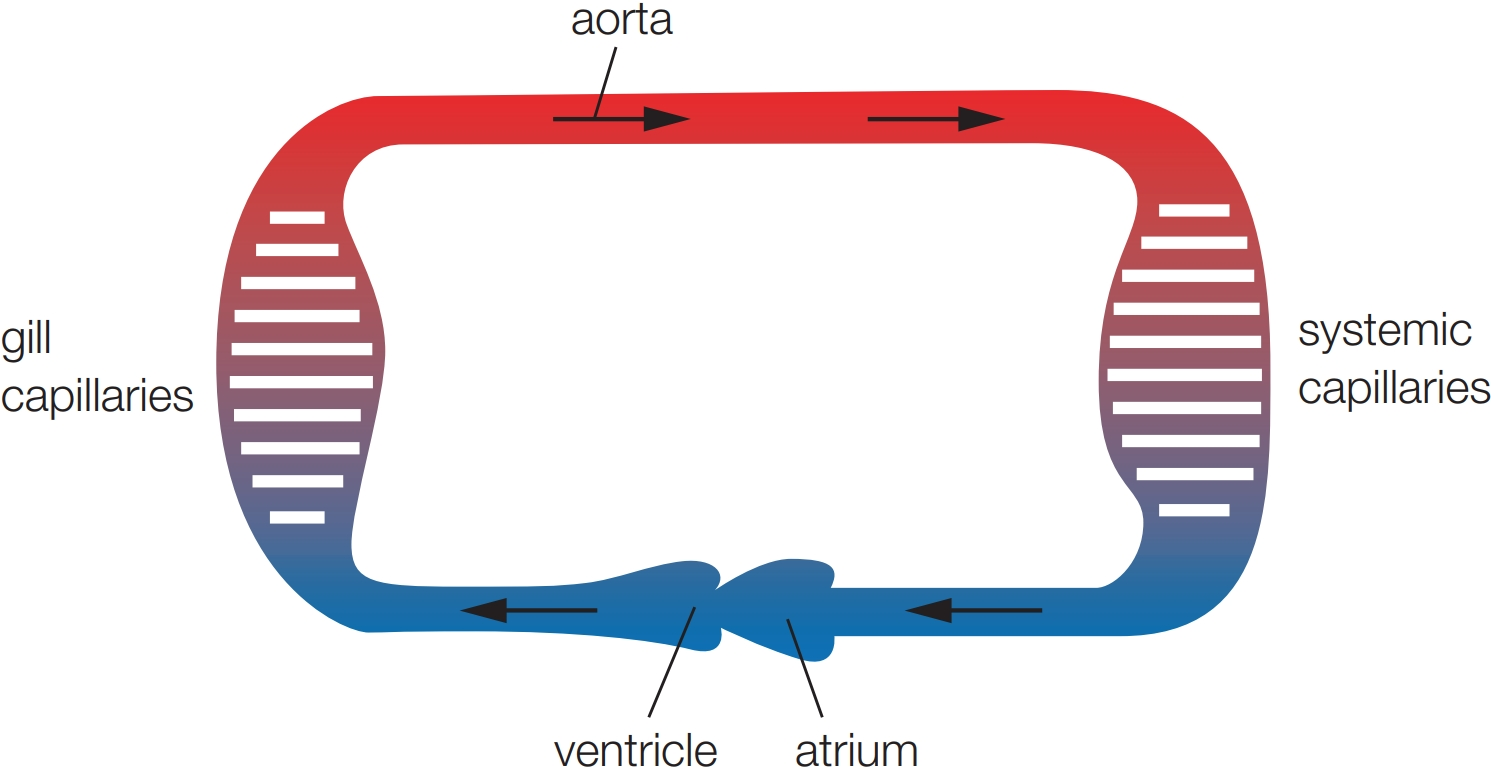
\includegraphics[scale=0.15]{Biology/1B/Images/1B-1-1.png}
            \caption{The single circulation of a fish.}
        \end{figure}
    \end{itemize}
    \item[2.] \textbf{Double Circulation:}
    \begin{itemize}
        \item Blood passes through the heart twice per cycle.
        \begin{itemize}
            \item[a)] \textbf{Pulmonary Circulation:} Heart $\rightarrow$ Lungs $\rightarrow$ Heart.
            \item[b)] \textbf{Systemic Circulation:} Heart $\rightarrow$ Body $\rightarrow$ Heart.
        \end{itemize}
        \begin{figure}[H]
            \centering
            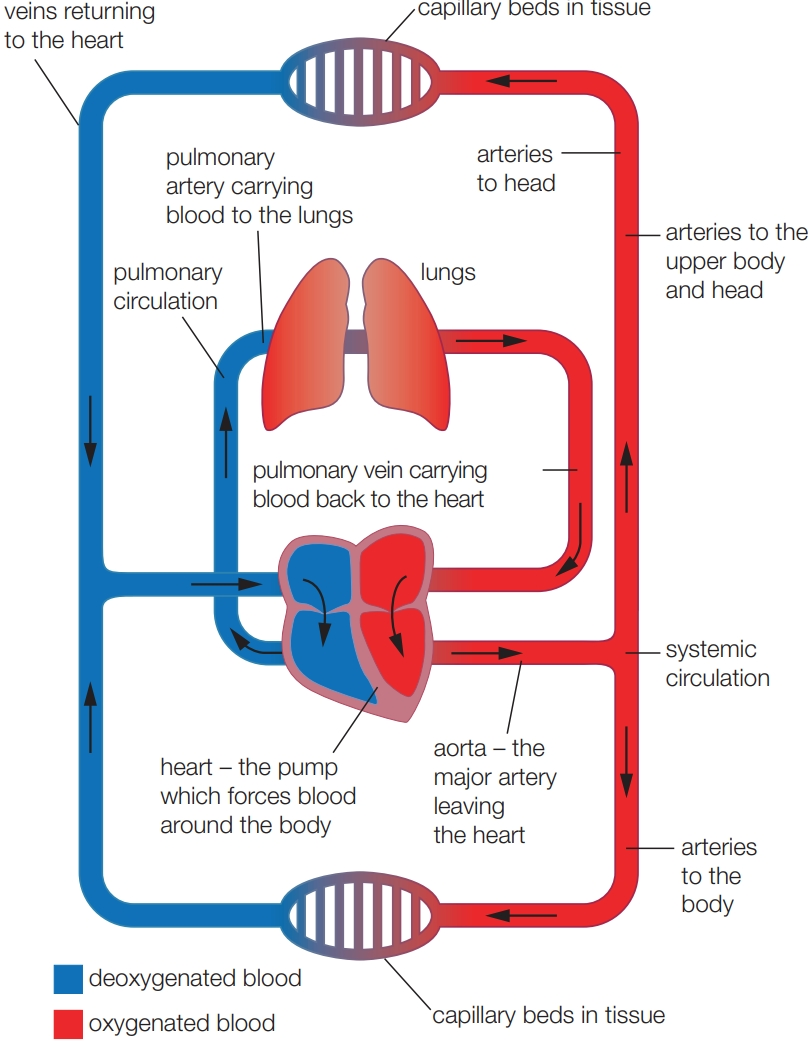
\includegraphics[scale=0.25]{Biology/1B/Images/1B-1-2.png}
            \caption{A double circulation sends blood at high pressure, carrying lots of oxygen, to the active cells of the body.
            Take note: this is a schematic diagram. In a real double circulation, all of the blood vessels enter and leave from
            the top of the heart.}
        \end{figure}
        \item Advantages:
        \begin{itemize}
            \item Maintain high blood pressure in systemic circulation.
            \item Efficient oxygen delivery to active tissues.
        \end{itemize}
    \end{itemize}
\end{itemize}